\documentclass{beamer}
\usepackage{ctex, hyperref}
\usepackage[T1]{fontenc}

% other packages
\usepackage{latexsym,amsmath,xcolor,multicol,booktabs,calligra,color}
\usepackage{graphicx,pstricks,listings,stackengine,subfigure}

\author{徐璨}
\title{基于扩散模型的三维分子设计}
\subtitle{毕业设计开题报告}
\institute{浙江工商大学 统计与数学学院}
\date{2023年3月15日}
\usepackage{zjgsu}
\setsansfont{Times New Roman}
\setmainfont{Times New Roman}

% defs
\def\cmd#1{\texttt{\color{red}\footnotesize $\backslash$#1}}
\def\env#1{\texttt{\color{blue}\footnotesize #1}}
\definecolor{deepblue}{rgb}{0,0,0.5}
\definecolor{deepred}{rgb}{0.6,0,0}
\definecolor{deepgreen}{rgb}{0,0.5,0}
\definecolor{halfgray}{gray}{0.55}

\lstset{
    basicstyle=\ttfamily\small,
    keywordstyle=\bfseries\color{deepblue},
    emphstyle=\ttfamily\color{deepred},    % Custom highlighting style
    stringstyle=\color{deepgreen},
    numbers=left,
    numberstyle=\small\color{halfgray},
    rulesepcolor=\color{red!20!green!20!blue!20},
    frame=shadowbox,
}


\begin{document}

\kaishu
\begin{frame}
    \titlepage
    \centering{导师:王伟刚 教授}
    \begin{figure}[htpb]
        \begin{center}
            
\includegraphics[width=0.15\linewidth]{figure/zjgsu} % 这个位置可能需要调整
        \end{center}
    \end{figure}
\end{frame}

\begin{frame}
    \tableofcontents[sectionstyle=show,subsectionstyle=show/shaded/hide,subsubsectionstyle=show/shaded/hide]
\end{frame}


\section{研究背景与意义}
\begin{frame}{研究背景}
    \begin{itemize}
        \item 近年来基于深度学习的生成模型也在多领域有成功应用,例如AI在图画、语音、视频、对话等应用上的优秀表现引发了社会对人工智能新一轮广泛关注与热烈讨论。
        \item 在智能计算的计算医药相关研究中,深度学习模型在药物发现、药物属性预测等应用中已经展现出良好的性能和极大的潜力。人工智能技术应用能够为药物研发的多个阶段降本增效。过去的2022年,AI制药赛道相关融资总金额达百亿美元。国内互联网巨头如百度百图生科、华为EIHealth、腾讯云深智药,及初创企业晶泰科技,剂泰医药,星药科技等,相关成果已经展现出深度学习在该领域的强大性能和广阔前景。
    \end{itemize}
\end{frame}

\begin{frame}{研究意义}
    \begin{itemize}
        \item 近来大火的生成模型被广泛应用于智能计算领域,人工智能算法有望根据人类的要求生成理想的结果,帮助提升药物发现与设计的效率与质量。
        \item 在计算化学的相关研究中,深度学习模型的成功落地能够推动制药企业减少湿实验成本,助力靶点确认、药物发现、分子生成、化学反应设计、化合物筛选、临床试验、风险评估等多阶段。
        \item 本文聚焦于深度学习算法在三维药物分子发现这一主题,意在利用时下最优的生成模型算法,创新性设计出更符合三位药物理化性质的算法,提升全新药物分子设计的性能与效率。
    \end{itemize}
\end{frame}


% \begin{frame}{为什么需要Beamer}
%     \begin{itemize}[<+-| alert@+>] % 当然,除了alert,手动在里面插 \pause 也行
%         \item 大家都会\LaTeX{},好多学校都有自己的Beamer主题
%         \item 中文支持请选择 Xe\LaTeX{} 编译选项
%         \item Overleaf项目地址位于 \url{https://www.overleaf.com/latex/templates/thu-beamer-theme/vwnqmzndvwyb},可以直接使用
%         \item GitHub项目地址位于 \url{https://github.com/Trinkle23897/THU-Beamer-Theme},如果有bug或者feature request可以去里面提issue
%     \end{itemize}
% \end{frame}


\section{国内外研究现状}
\begin{frame}{生成模型}
    \begin{itemize}
        \item 生成模型近年来在作画、视频创作、空间建模、文本生成等多方面都有了成功的应用。早期的生成模型研究主要集中在变分自编码器(VAE)、生成对抗网络(GAN)、流型模型(Flow-based models)、自回归模型(Auto-regressive models)及深度强化学习领域。近两年来,基于扩散模型的生成模型(Diffusion-based models)以其优异的性能、计算资源消耗相对较少在学术圈与工业界爆火。
        \item 相关Diffusion模型的研究包括对干扰、去噪过程的改进(DDPMs,SGMs,Score SDEs),采样策略的改进,损失函数,各类型数据应用(计算机视觉、自然语言处理、时序建模、信号传递、多模态学习、图建模、医学影像)等。
    \end{itemize}
\end{frame}

\begin{frame}{计算医药}
    \begin{itemize}
        \item 生成模型的发展也带动了其在智能计算领域的应用。5年前,药物分子、蛋白质配体分子等分子学习任务主要聚焦于2D分子结构,但实际上,分子结构信息远不止原子间的拓扑结构信息这么简单,因此某一分子在自然界中可能存在种类繁多的同分异构体,故近来对分子的研究拓展到了结合3D信息对不同分子构型的相关研究。因此在3D分子生成任务上,目标不再是生成简单的可能有效的分子,更要生成具备理想属性和性质稳定的分子3D构型。
        \item 3D分子生成任务又可分为3D构型生成与全新分子生成。3D构型生成的目标是根据给定的分子式,生成理想的三维构型。全新分子生成的目标则是凭空生成全新的、有效的分子。
        \item 3D构型生成的研究有基于VAE的CVGAE,GraphDG,ConfVAE,基于扩散模型的ConfGF,EVFN,GeoDiff等。
    \end{itemize}
\end{frame}
\begin{frame}{计算医药}
    \begin{itemize}
        \item 2D分子生成的研究有基于VAE的TransVAE,JT-VAE,基于GAN的MolGAN,基于Flow和AR的GraphDF,GraphAF,MoFlow,基于能量函数的GraphEBM等。
        \item 3D分子生成的研究有基于AR的G-SchNet,GEN3D,基于Flow的E-NFs,G-SphereNet,基于强化学习的MolGym,基于VAE的3DMolNet。基于这些模型的算法存在着计算需求大,效果有限的问题。
        \item 目前基于Diffusion的3D分子生成模型仅有两个,EDM(ICML-22)\cite{edm_icml_hoogeboom_22}和MDM(AAAI-22)\cite{mdm_aaai_huang_22}在扩散模型的内核设计上仍沿用了之前研究的设计如SchNet\cite{schnet_schutt_17}等,本人认为传统的图网络在空间几何建模上存在劣势,且不符合扩散模型的内在机理。
    \end{itemize}
\end{frame}

\section{研究内容}
\begin{frame}{前期准备}
    \begin{itemize}
        \item \textcolor[rgb]{0.827,0.318,0.298}{本文意在利用生成模型,提出创新的算法,生成全新且有效的分子。}
        \item 本文首先选取GEOM-QM9和GEOM-Drugs作为研究数据集。GEOM-QM9包含130831个分子,平均每个分子由19个分子构成。
        \item GEOM-Drugs包含超过600W个分子构型,将每个分子的不同构型经过筛选后,处理得到29W个稳定的分子构型,平均每个分子由44个原子构成。
    \end{itemize}
\end{frame}

\begin{frame}{生成模型构建}
    \begin{itemize}
        \item 本文基于DDPMs构建分子生成模型框架,包括扩散过程与去噪过程。
        \item 扩散过程本质是通过给初始数据有规律地增加噪声,使其经过$T$时间步后收敛至高斯噪声。
        \item 去噪过程的本质是通过设计的去噪神经网络内核,将高斯噪声还原至初始状态,使其与初始数据相似。
    \end{itemize}
\end{frame}

\begin{frame}{等变图网络构建}
    \begin{itemize}
        \item 之前的研究基于的图网络基本比较简单,如SchNet\cite{schnet_schutt_17}。
        \item 先前的图网络对于3D几何信息的建模能力有限,且不符合扩散模型的内在本质。本文提出运用全局注意力机制代替图卷积,对3D几何信息进行建模。
        \item 本文等变图网络对三维空间信息的建模分为两个并行模块:inter-atomic级别的和pair-wise级别的。在每个Interblock中,两个并行模块分别对原子和原子对的特征通过全局注意力机制进行学习,并通过交换模块对信息进行统一。
    \end{itemize}
\end{frame}

\begin{frame}{生成过程示例}
    \begin{figure}[H]
        \centering
        \subfigure{
            \label{014}
            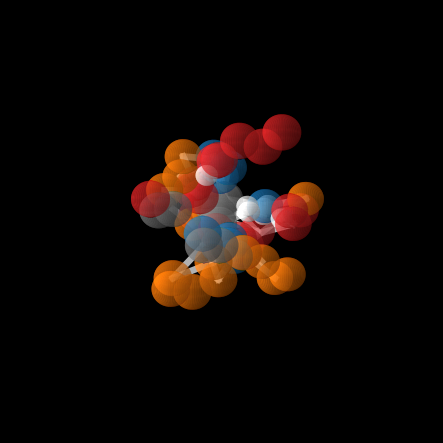
\includegraphics[width=0.13\linewidth]{figure/chain_014.png}
        }
        \hspace{0mm}
        \subfigure{
            \label{040}
            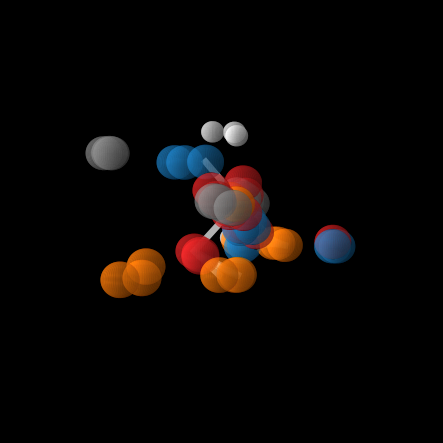
\includegraphics[width=0.13\linewidth]{figure/chain_040.png}
        }
        \hspace{0mm}
        \subfigure{
            \label{050}
            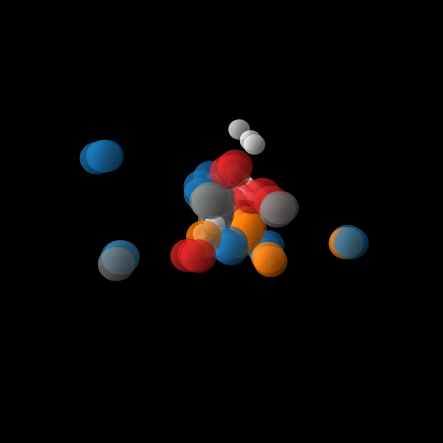
\includegraphics[width=0.13\linewidth]{figure/chain_050.png}
        }
        \hspace{0mm}
        \subfigure{
            \label{065}
            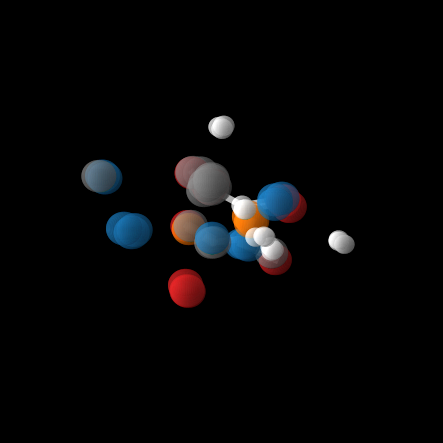
\includegraphics[width=0.13\linewidth]{figure/chain_065.png}
        }
        \hspace{0mm}
        \subfigure{
            \label{072}
            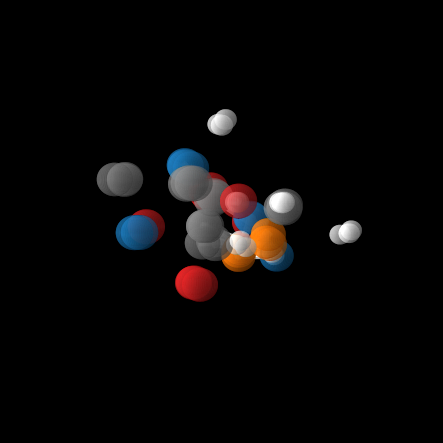
\includegraphics[width=0.13\linewidth]{figure/chain_072.png}
        }
        \hspace{0mm}
        \subfigure{
            \label{077}
            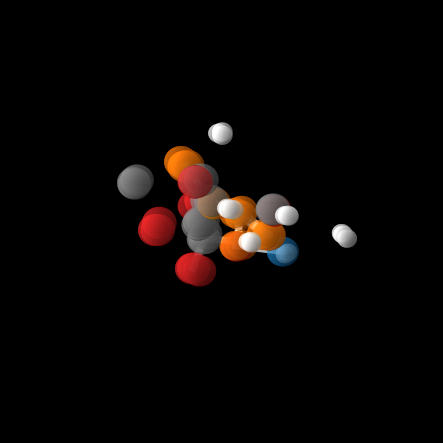
\includegraphics[width=0.13\linewidth]{figure/chain_077.png}
        }
        \hspace{0mm}
        \subfigure{
            \label{082}
            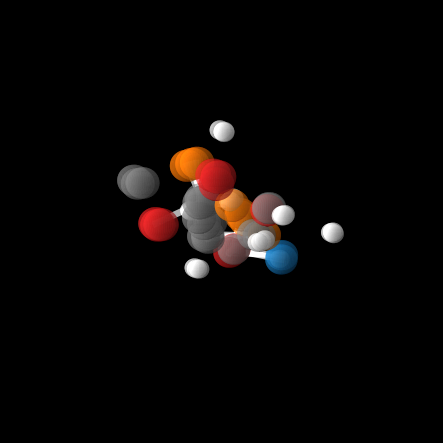
\includegraphics[width=0.13\linewidth]{figure/chain_082.png}
        }
        \hspace{0mm}
        \subfigure{
            \label{086}
            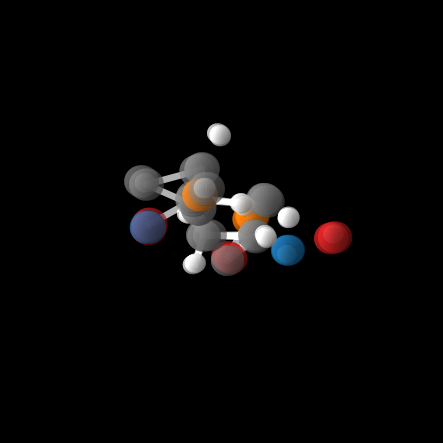
\includegraphics[width=0.13\linewidth]{figure/chain_086.png}
        }
        \hspace{0mm}
        \subfigure{
            \label{089}
            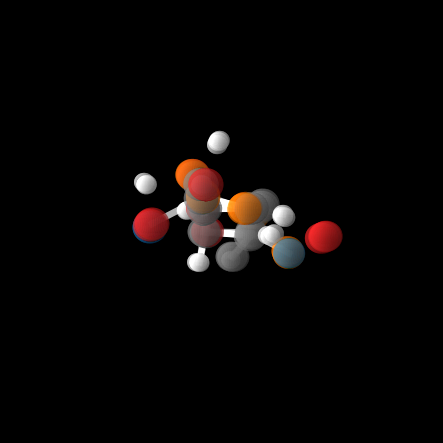
\includegraphics[width=0.13\linewidth]{figure/chain_089.png}
        }
        \hspace{0mm}
        \subfigure{
            \label{091}
            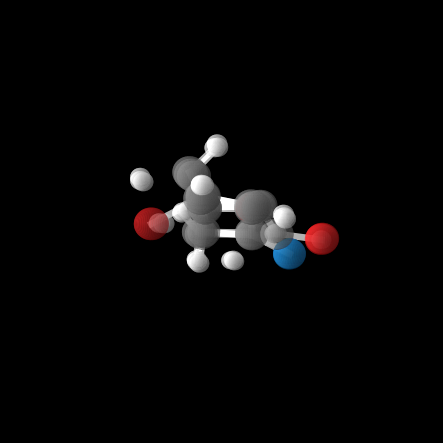
\includegraphics[width=0.13\linewidth]{figure/chain_091.png}
        }
        \hspace{0mm}
        \subfigure{
            \label{093}
            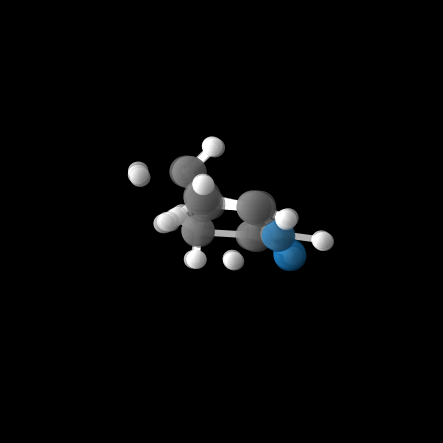
\includegraphics[width=0.13\linewidth]{figure/chain_093.png}
        }
        \hspace{0mm}
        \subfigure{
            \label{107}
            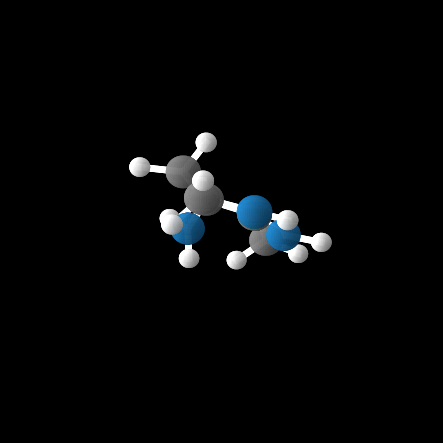
\includegraphics[width=0.13\linewidth]{figure/chain_107.png}
        }
        \caption{生成流程示意图 “CNC1=C(N)CCN1”}
        \label{gen_illustration}
    \end{figure}
    \begin{figure}[H]
        \centering
        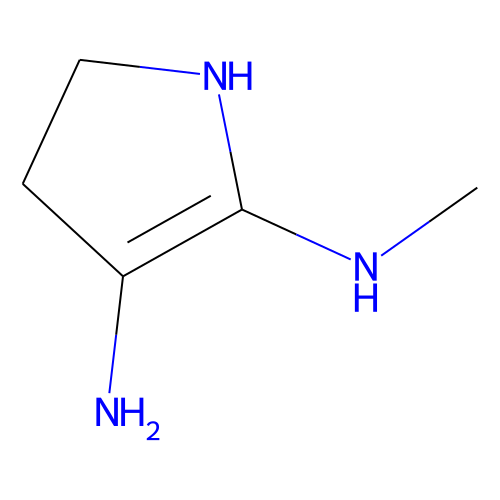
\includegraphics[width=0.15\linewidth]{figure/[H]N([H])C1=C(N([H])C([H])([H])[H])N([H])C([H])([H])C1([H])[H].png}
        \caption{分子“CNC1=C(N)CCN1”理论结构}
    \end{figure}
\end{frame}


\begin{frame}{生成结果示例}
    \begin{figure}[H]
        \centering
        \subfigure{
            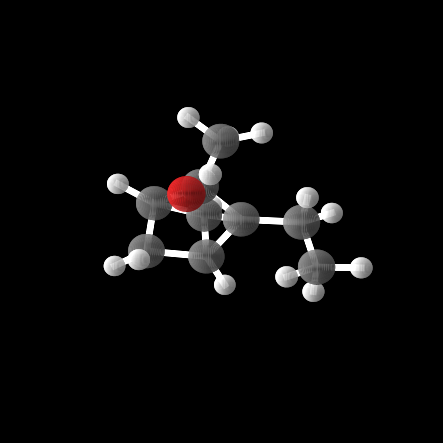
\includegraphics[width=0.13\linewidth]{figure/stable/qm9_02-23-03-02-19molecule_002.png}
        }
        \hspace{0mm}
        \subfigure{
            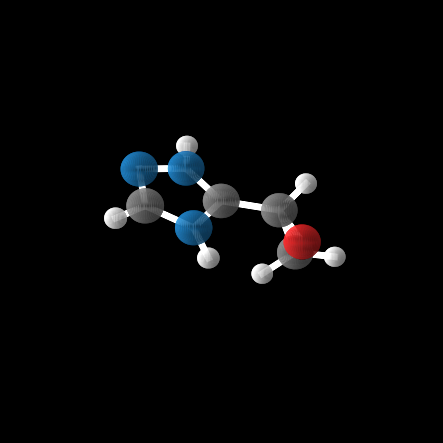
\includegraphics[width=0.13\linewidth]{figure/stable/qm9_02-23-03-02-19molecule_006.png}
        }
        \hspace{0mm}
        \subfigure{
            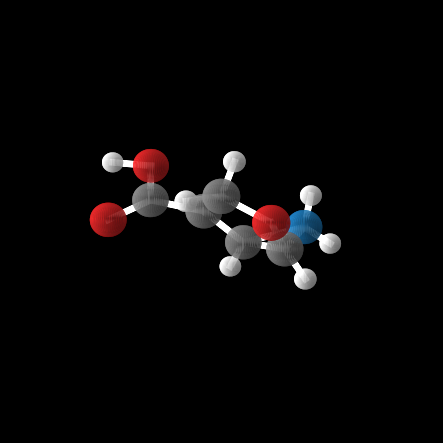
\includegraphics[width=0.13\linewidth]{figure/stable/qm9_02-23-03-02-19molecule_017.png}
        }
        \hspace{0mm}
        \subfigure{
            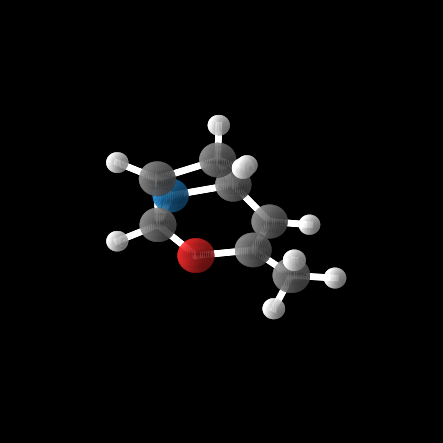
\includegraphics[width=0.13\linewidth]{figure/stable/qm9_02-23-03-02-19molecule_023.png}
        }
        \hspace{0mm}
        \subfigure{
            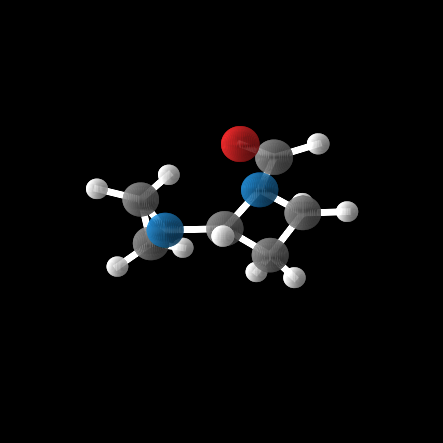
\includegraphics[width=0.13\linewidth]{figure/stable/qm9_02-23-03-02-19molecule_028.png}
        }
        \hspace{0mm}
        \subfigure{
            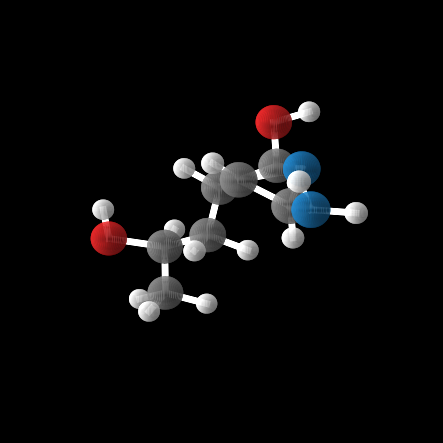
\includegraphics[width=0.13\linewidth]{figure/stable/qm9_02-23-03-02-19molecule_029.png}
        }
        \hspace{0mm}
        \subfigure{
            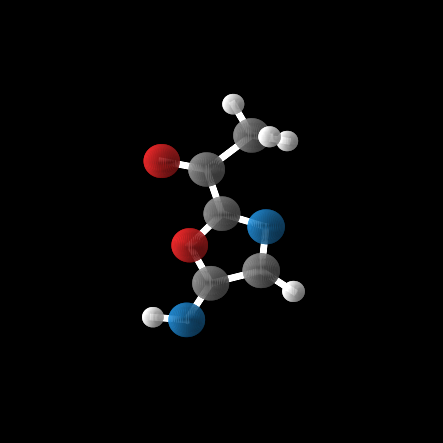
\includegraphics[width=0.13\linewidth]{figure/stable/qm9_02-23-03-02-19molecule_030.png}
        }
        \hspace{0mm}
        \subfigure{
            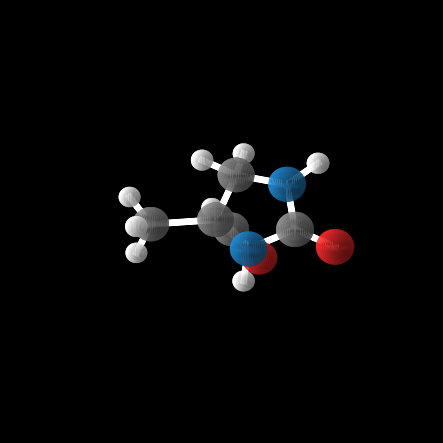
\includegraphics[width=0.13\linewidth]{figure/stable/qm9_02-23-03-02-19molecule_032.png}
        }
        \hspace{0mm}
        \subfigure{
            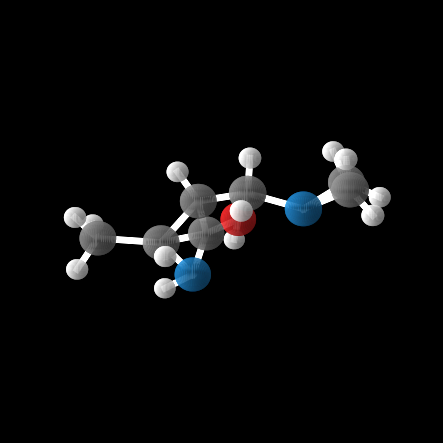
\includegraphics[width=0.13\linewidth]{figure/stable/qm9_02-23-03-02-19molecule_035.png}
        }
        \hspace{0mm}
        \subfigure{
            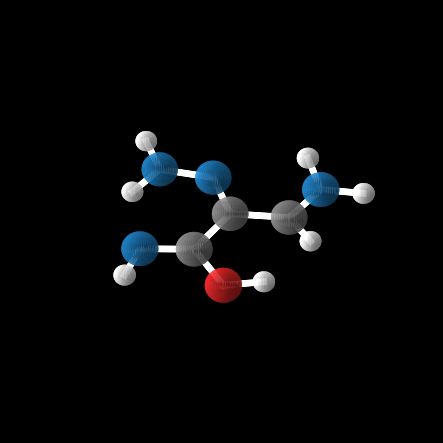
\includegraphics[width=0.13\linewidth]{figure/stable/qm9_02-23-03-02-19molecule_036.png}
        }
        \hspace{0mm}
        \subfigure{
            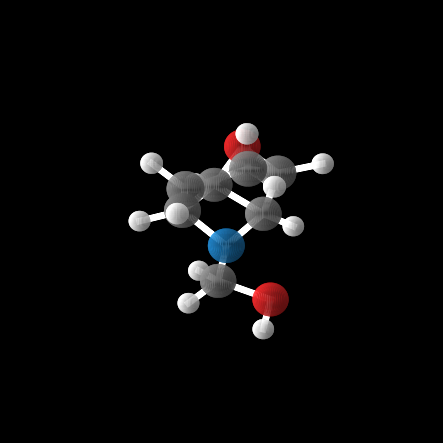
\includegraphics[width=0.13\linewidth]{figure/stable/qm9_02-23-03-02-19molecule_040.png}
        }
        \hspace{0mm}
        \subfigure{
            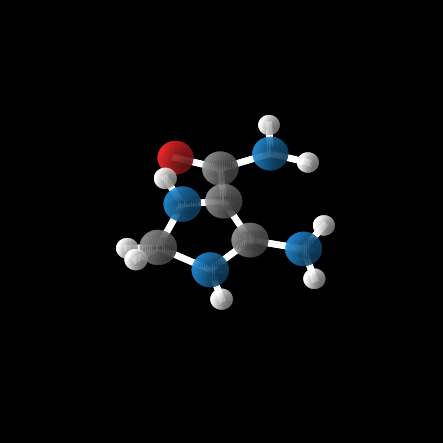
\includegraphics[width=0.13\linewidth]{figure/stable/qm9_02-23-03-02-19molecule_042.png}
        }
        \hspace{0mm}
        \subfigure{
            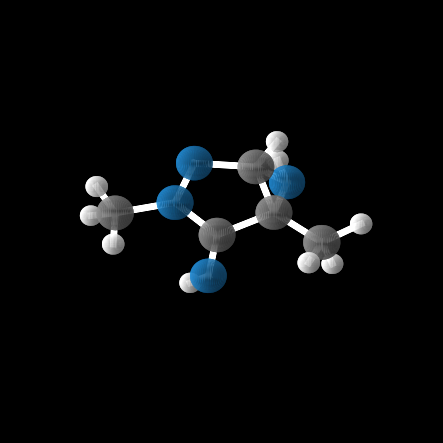
\includegraphics[width=0.13\linewidth]{figure/stable/qm9_02-23-03-02-19molecule_045.png}
        }
        \hspace{0mm}
        \subfigure{
            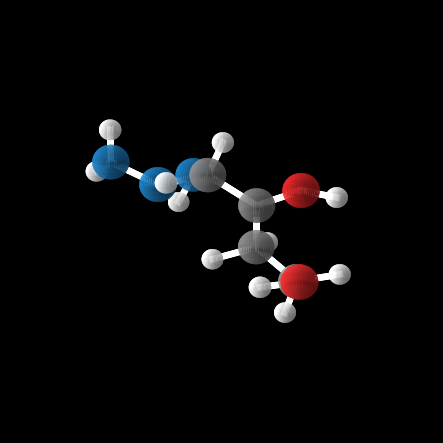
\includegraphics[width=0.13\linewidth]{figure/stable/qm9_02-23-03-02-19molecule_046.png}
        }
        \hspace{0mm}
        \subfigure{
            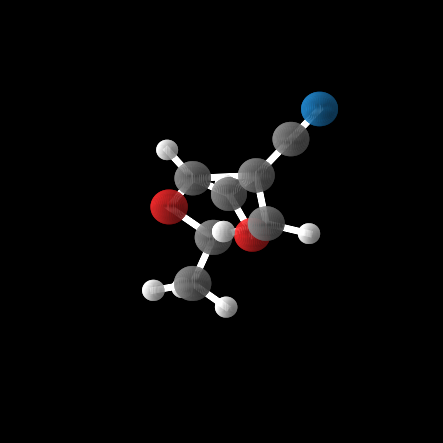
\includegraphics[width=0.13\linewidth]{figure/stable/qm9_02-23-03-02-19molecule_048.png}
        }
        \hspace{0mm}
        \subfigure{
            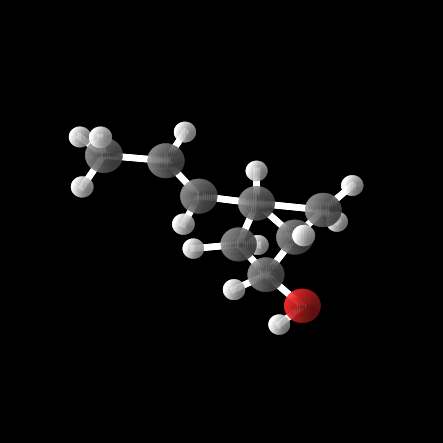
\includegraphics[width=0.13\linewidth]{figure/stable/qm9_02-23-03-02-19molecule_051.png}
        }
        \hspace{0mm}
        \subfigure{
            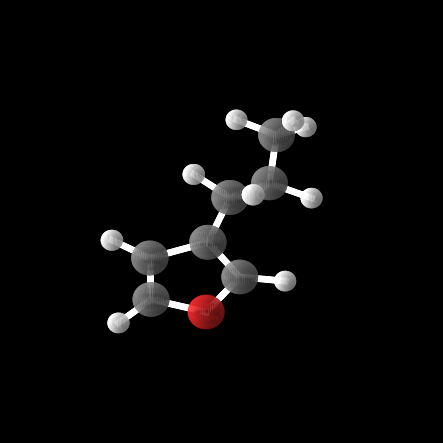
\includegraphics[width=0.13\linewidth]{figure/stable/qm9_02-23-03-02-19molecule_052.png}
        }
        \hspace{0mm}
        \subfigure{
            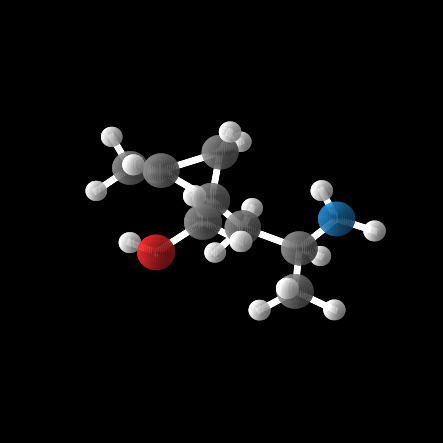
\includegraphics[width=0.13\linewidth]{figure/stable/qm9_02-23-03-02-19molecule_058.png}
        }
        \hspace{0mm}
        \subfigure{
            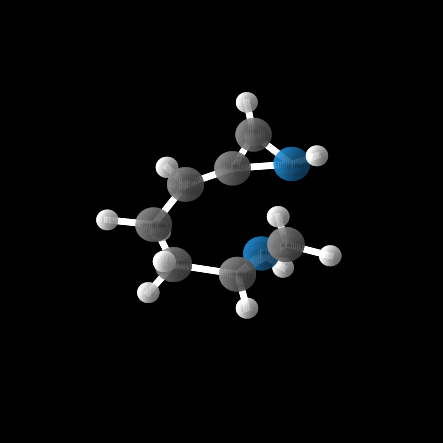
\includegraphics[width=0.13\linewidth]{figure/stable/qm9_02-23-03-02-19molecule_065.png}
        }
        \hspace{0mm}
        \subfigure{
            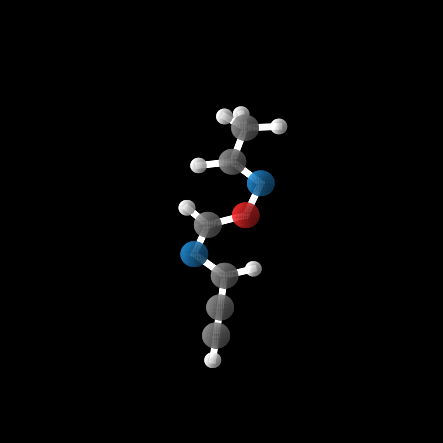
\includegraphics[width=0.13\linewidth]{figure/stable/qm9_02-23-03-02-19molecule_066.png}
        }
        \hspace{0mm}
        \subfigure{
            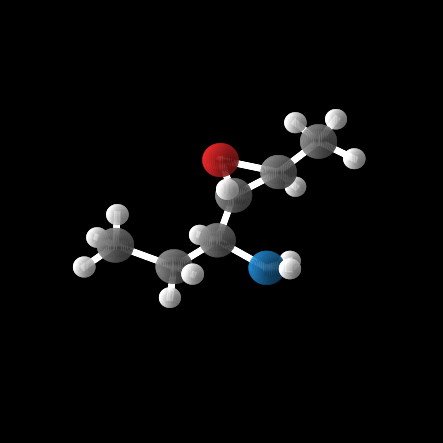
\includegraphics[width=0.13\linewidth]{figure/stable/qm9_02-23-03-02-19molecule_086.png}
        }
        \hspace{0mm}
        \subfigure{
            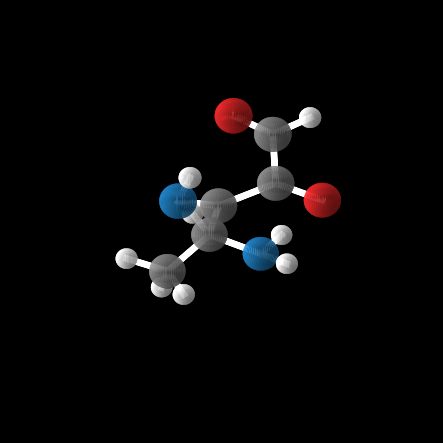
\includegraphics[width=0.13\linewidth]{figure/stable/qm9_02-23-03-02-19molecule_091.png}
        }
        \hspace{0mm}
        \subfigure{
            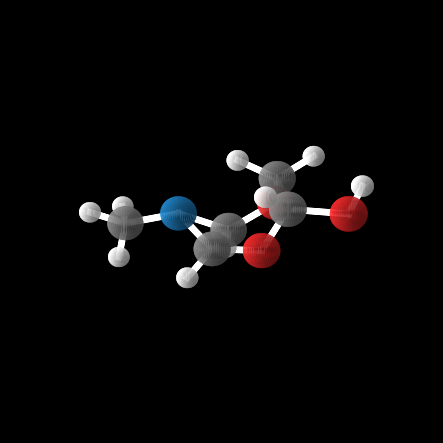
\includegraphics[width=0.13\linewidth]{figure/stable/qm9_02-23-03-02-19molecule_097.png}
        }
        \hspace{0mm}
        \subfigure{
            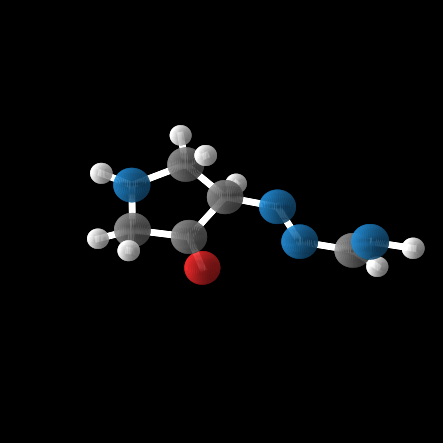
\includegraphics[width=0.13\linewidth]{figure/stable/qm9_02-23-03-02-19molecule_098.png}
        }
        \hspace{0mm}
        \caption{生成分子示例}
    \end{figure}
\end{frame}

\section{计划进度}
\begin{frame}
    \begin{itemize}
        \item 2023.01-2023.03:前期调研与相关文献阅读
        \item 2023.03-2023.04:模型搭建
        \item 2023.04-2023.05:模型训练,性能调优与对比试验
        \item 2023.05-2023.07:文章撰写
        \item 2023.07-2023.09:文章修改
    \end{itemize}
\end{frame}

% \begin{frame}{这一份主题目前与THU Beamer Theme区别在于}
%     \begin{itemize}
%         \item 修改校徽
%         \item 修改主题色
%     \end{itemize}
% \end{frame}

% \begin{frame}{Why Beamer}
%     \begin{itemize}
%         \item \LaTeX 广泛用于学术界,期刊会议论文模板
%     \end{itemize}
%     \begin{table}[h]
%         \centering
%         \begin{tabular}{c|c}
%             Microsoft\textsuperscript{\textregistered}  Word & \LaTeX \\
%             \hline
%             文字处理工具 & 专业排版软件 \\
%             容易上手,简单直观 & 容易上手 \\
%             所见即所得 & 所见即所想,所想即所得 \\
%             高级功能不易掌握 & 进阶难,但一般用不到 \\
%             处理长文档需要丰富经验 & 和短文档处理基本无异 \\
%             花费大量时间调格式 & 无需担心格式,专心作者内容 \\
%             公式排版差强人意 & 尤其擅长公式排版 \\
%             二进制格式,兼容性差 & 文本文件,易读、稳定 \\
%             付费商业许可 & 自由免费使用 \\
%         \end{tabular}
%     \end{table}
% \end{frame}

% \begin{frame}{排版举例}
%     \begin{exampleblock}{无编号公式} % 加 * 
%         \begin{equation*}
%             J(\theta) = \mathbb{E}_{\pi_\theta}[G_t] = \sum_{s\in\mathcal{S}} d^\pi (s)V^\pi(s)=\sum_{s\in\mathcal{S}} d^\pi(s)\sum_{a\in\mathcal{A}}\pi_\theta(a|s)Q^\pi(s,a)
%         \end{equation*}
%     \end{exampleblock}
%     \begin{exampleblock}{多行多列公式\footnote{如果公式中有文字出现,请用 $\backslash$mathrm\{\} 或者 $\backslash$text\{\} 包含,不然就会变成 $clip$,在公式里看起来比 $\mathrm{clip}$ 丑非常多。}}
%         % 使用 & 分隔
%         \begin{align}
%             Q_\mathrm{target}&=r+\gamma Q^\pi(s^\prime, \pi_\theta(s^\prime)+\epsilon)\\
%             \epsilon&\sim\mathrm{clip}(\mathcal{N}(0, \sigma), -c, c)\nonumber
%         \end{align}
%     \end{exampleblock}
% \end{frame}

% \begin{frame}
%     \begin{exampleblock}{编号多行公式}
%         % Taken from Mathmode.tex
%         \begin{multline}
%             A=\lim_{n\rightarrow\infty}\Delta x\left(a^{2}+\left(a^{2}+2a\Delta x+\left(\Delta x\right)^{2}\right)\right.\label{eq:reset}\\
%             +\left(a^{2}+2\cdot2a\Delta x+2^{2}\left(\Delta x\right)^{2}\right)\\
%             +\left(a^{2}+2\cdot3a\Delta x+3^{2}\left(\Delta x\right)^{2}\right)\\
%             +\ldots\\
%             \left.+\left(a^{2}+2\cdot(n-1)a\Delta x+(n-1)^{2}\left(\Delta x\right)^{2}\right)\right)\\
%             =\frac{1}{3}\left(b^{3}-a^{3}\right)
%         \end{multline}
%     \end{exampleblock}
% \end{frame}

% \begin{frame}{图形与分栏}
%     % From thuthesis user guide.
%     \begin{minipage}[c]{0.3\linewidth}
%         \psset{unit=0.8cm}
%         \begin{pspicture}(-1.75,-3)(3.25,4)
%             \psline[linewidth=0.25pt](0,0)(0,4)
%             \rput[tl]{0}(0.2,2){$\vec e_z$}
%             \rput[tr]{0}(-0.9,1.4){$\vec e$}
%             \rput[tl]{0}(2.8,-1.1){$\vec C_{ptm{ext}}$}
%             \rput[br]{0}(-0.3,2.1){$\theta$}
%             \rput{25}(0,0){%
%             \psframe[fillstyle=solid,fillcolor=lightgray,linewidth=.8pt](-0.1,-3.2)(0.1,0)}
%             \rput{25}(0,0){%
%             \psellipse[fillstyle=solid,fillcolor=yellow,linewidth=3pt](0,0)(1.5,0.5)}
%             \rput{25}(0,0){%
%             \psframe[fillstyle=solid,fillcolor=lightgray,linewidth=.8pt](-0.1,0)(0.1,3.2)}
%             \rput{25}(0,0){\psline[linecolor=red,linewidth=1.5pt]{->}(0,0)(0.,2)}
% %           \psRotation{0}(0,3.5){$\dot\phi$}
% %           \psRotation{25}(-1.2,2.6){$\dot\psi$}
%             \psline[linecolor=red,linewidth=1.25pt]{->}(0,0)(0,2)
%             \psline[linecolor=red,linewidth=1.25pt]{->}(0,0)(3,-1)
%             \psline[linecolor=red,linewidth=1.25pt]{->}(0,0)(2.85,-0.95)
%             \psarc{->}{2.1}{90}{112.5}
%             \rput[bl](.1,.01){C}
%         \end{pspicture}
%     \end{minipage}\hspace{1cm}
%     \begin{minipage}{0.5\linewidth}
%         \medskip
%         %\hspace{2cm}
%         \begin{figure}[h]
%             \centering
%             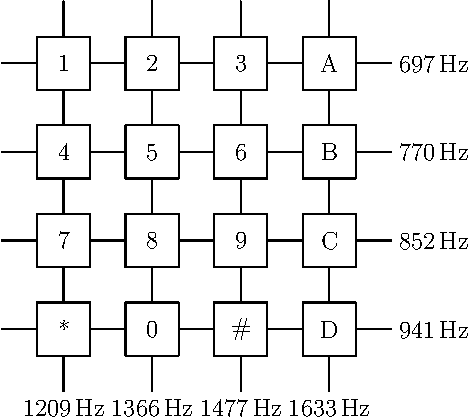
\includegraphics[height=.4\textheight]{figure/dtmf.pdf}
%         \end{figure}
%     \end{minipage}
% \end{frame}

% \begin{frame}[fragile]{\LaTeX{} 常用命令}
%     \begin{exampleblock}{命令}
%         \centering
%         \footnotesize
%         \begin{tabular}{llll}
%             \cmd{chapter} & \cmd{section} & \cmd{subsection} & \cmd{paragraph} \\
%             章 & 节 & 小节 & 带题头段落 \\\hline
%             \cmd{centering} & \cmd{emph} & \cmd{verb} & \cmd{url} \\
%             居中对齐 & 强调 & 原样输出 & 超链接 \\\hline
%             \cmd{footnote} & \cmd{item} & \cmd{caption} & \cmd{includegraphics} \\
%             脚注 & 列表条目 & 标题 & 插入图片 \\\hline
%             \cmd{label} & \cmd{cite} & \cmd{ref} \\
%             标号 & 引用参考文献 & 引用图表公式等\\\hline
%         \end{tabular}
%     \end{exampleblock}
%     \begin{exampleblock}{环境}
%         \centering
%         \footnotesize
%         \begin{tabular}{lll}
%             \env{table} & \env{figure} & \env{equation}\\
%             表格 & 图片 & 公式 \\\hline
%             \env{itemize} & \env{enumerate} & \env{description}\\
%             无编号列表 & 编号列表 & 描述 \\\hline
%         \end{tabular}
%     \end{exampleblock}
% \end{frame}

% \begin{frame}[fragile]{\LaTeX{} 环境命令举例}
%     \begin{minipage}{0.5\linewidth}
% \begin{lstlisting}[language=TeX]
% \begin{itemize}
%   \item A \item B
%   \item C
%   \begin{itemize}
%     \item C-1
%   \end{itemize}
% \end{itemize}
% \end{lstlisting}
%     \end{minipage}\hspace{1cm}
%     \begin{minipage}{0.3\linewidth}
%         \begin{itemize}
%             \item A
%             \item B
%             \item C
%             \begin{itemize}
%                 \item C-1
%             \end{itemize}
%         \end{itemize}
%     \end{minipage}
%     \medskip
%     \pause
%     \begin{minipage}{0.5\linewidth}
% \begin{lstlisting}[language=TeX]
% \begin{enumerate}
%   \item 巨佬 \item 大佬
%   \item 萌新
%   \begin{itemize}
%     \item[n+e] 瑟瑟发抖
%   \end{itemize}
% \end{enumerate}
% \end{lstlisting}
%     \end{minipage}\hspace{1cm}
%     \begin{minipage}{0.3\linewidth}
%         \begin{enumerate}
%             \item 巨佬
%             \item 大佬
%             \item 萌新
%             \begin{itemize}
%                 \item[n+e] 瑟瑟发抖
%             \end{itemize}
%         \end{enumerate}
%     \end{minipage}
% \end{frame}

% \begin{frame}[fragile]{\LaTeX{} 数学公式}
%     \begin{columns}
%         \begin{column}{.55\textwidth}
% \begin{lstlisting}[language=TeX]
% $V = \frac{4}{3}\pi r^3$

% \[
%   V = \frac{4}{3}\pi r^3
% \]

% \begin{equation}
%   \label{eq:vsphere}
%   V = \frac{4}{3}\pi r^3
% \end{equation}
% \end{lstlisting}
%         \end{column}
%         \begin{column}{.4\textwidth}
%             $V = \frac{4}{3}\pi r^3$
%             \[
%                 V = \frac{4}{3}\pi r^3
%             \]
%             \begin{equation}
%                 \label{eq:vsphere}
%                 V = \frac{4}{3}\pi r^3
%             \end{equation}
%         \end{column}
%     \end{columns}
%     \begin{itemize}
%         \item 更多内容请看 \href{https://zh.wikipedia.org/wiki/Help:数学公式}{\color{purple}{这里}}
%     \end{itemize}
% \end{frame}

% \begin{frame}[fragile]
%     \begin{columns}
%         \column{.6\textwidth}
% \begin{lstlisting}[language=TeX]
%     \begin{table}[htbp]
%       \caption{编号与含义}
%       \label{tab:number}
%       \centering
%       \begin{tabular}{cl}
%         \toprule
%         编号 & 含义 \\
%         \midrule
%         1 & 4.0 \\
%         2 & 3.7 \\
%         \bottomrule
%       \end{tabular}
%     \end{table}
%     公式~(\ref{eq:vsphere}) 的
%     编号与含义请参见
%     表~\ref{tab:number}。
% \end{lstlisting}
%         \column{.4\textwidth}
%         \begin{table}[htpb]
%             \centering
%             \caption{编号与含义}
%             \label{tab:number}
%             \begin{tabular}{cl}\toprule
%                 编号 & 含义 \\\midrule
%                 1 & 4.0\\
%                 2 & 3.7\\\bottomrule
%             \end{tabular}
%         \end{table}
%         \normalsize 公式~(\ref{eq:vsphere})的编号与含义请参见表~\ref{tab:number}。
%     \end{columns}
% \end{frame}

% \begin{frame}{作图}
%     \begin{itemize}
%         \item 矢量图 eps, ps, pdf
%         \begin{itemize}
%             \item METAPOST, pstricks, pgf $\ldots$
%             \item Xfig, Dia, Visio, Inkscape $\ldots$
%             \item Matlab / Excel 等保存为 pdf
%         \end{itemize}
%         \item 标量图 png, jpg, tiff $\ldots$
%         \begin{itemize}
%             \item 提高清晰度,避免发虚
%             \item 应尽量避免使用
%         \end{itemize}
%     \end{itemize}
%     \begin{figure}[htpb]
%         \centering
%         
\includegraphics[width=0.2\linewidth]{figure/zjgsu.jpg}
%         \caption{这个校徽就是矢量图}
%     \end{figure}
% \end{frame}






\section{参考文献}
\begin{frame}[allowframebreaks]
    \bibliography{ref}
    \tiny\bibliographystyle{siam}
    % 如果参考文献太多的话,可以像下面这样调整字体:
    % \tiny\bibliographystyle{alpha}
\end{frame}

\begin{frame}
    \begin{center}
        {\Huge\calligra Thanks!}
    \end{center}
\end{frame}

\end{document}